\documentclass[11pt,a4paper]{article}

% ------------------------------------------------------------------
% TALA research paper - revised to the four-stage backend
% Compile with: pdflatex tala_revised_research_paper.tex (twice)
% Remaining red [ ... ] items are values that must be copied from the
% final backend artifacts (ik_report.json, gravity_analysis.json, etc.)
% or verified against official NASA metadata before submission.
% Figures: place exported images in ./figures/ using the file names
% given in each \figorbox call; a labelled box is shown if a file is missing.
% ------------------------------------------------------------------

\usepackage[margin=1in]{geometry}
\usepackage[T1]{fontenc}
\usepackage{lmodern}
\usepackage{microtype}
\usepackage{amsmath,amssymb,mathtools}
\usepackage{graphicx}
\usepackage{booktabs}
\usepackage{array}
\usepackage{tabularx}
\usepackage{siunitx}
\usepackage{float}
\usepackage{enumitem}
\usepackage{xcolor}
\usepackage{hyperref}
\usepackage{caption}
\usepackage{subcaption}
\usepackage{url}
\usepackage{tikz}
\usetikzlibrary{arrows.meta,positioning,shapes.geometric,fit,calc}

\hypersetup{
  colorlinks=true,
  linkcolor=blue!45!black,
  citecolor=blue!45!black,
  urlcolor=blue!55!black,
  pdftitle={TALA: An Exploratory Framework for Astronaut Exercise Movement Analysis Using Computer Vision, OpenSim Kinematic Reconstruction, and NASA-Literature-Grounded Retrieval},
  pdfauthor={[Author Name]}
}
\sisetup{per-mode=symbol}
\setlength{\parskip}{0.35em}
\setlength{\emergencystretch}{2em}
\setlength{\parindent}{1.2em}
\renewcommand{\arraystretch}{1.15}

\newcommand{\TALA}{\textsc{TALA}}
\newcommand{\OpenSim}{\textsc{OpenSim}}
\newcommand{\MediaPipe}{\textsc{MediaPipe}}
\newcommand{\placeholder}[1]{{\color{red}\bfseries[#1]}}
\newcommand{\ins}{}

% Include a figure file if it exists, otherwise draw a labelled box.
\newcommand{\figorbox}[3][0.9\linewidth]{%
  \IfFileExists{figures/#2}{\includegraphics[width=#1]{figures/#2}}{%
  \fbox{\parbox[c][4.2cm][c]{\dimexpr#1-2\fboxsep-2\fboxrule\relax}{\centering\textcolor{red}{\textbf{Missing figure file}}\\[0.3em]
  \small\texttt{\detokenize{figures/#2}}\\[0.3em]\small #3}}}}

\tikzset{
  stage/.style={draw,rounded corners=3pt,thick,align=center,minimum width=3.0cm,minimum height=1.3cm,fill=blue!6,font=\small},
  data/.style={draw,rounded corners=1pt,align=center,minimum height=0.8cm,fill=gray!10,font=\footnotesize},
  arr/.style={-{Latex[length=2.2mm]},thick}
}

\title{\textbf{TALA: An Exploratory Framework for Astronaut Exercise Movement Analysis Using Computer Vision, OpenSim Kinematic Reconstruction, and NASA-Literature-Grounded Retrieval}}
\author{{Vince Aivan Rumalay}\\{Team O(1) - Solo}}
\date{November 2026}

\begin{document}
\maketitle

\begin{abstract}
Long-duration spaceflight exposes crew members to altered gravitational conditions that affect the mechanical environment in which exercise countermeasures are performed. Interpreting exercise recordings requires methods that can extract movement information, relate observed motion to a biomechanical model, and provide relevant scientific context. This paper presents \TALA\ (Twin-based Astronaut Life Analytics), an exploratory software framework integrating computer-vision-based pose estimation, \OpenSim\ kinematic reconstruction, biomechanical and movement analysis, and retrieval-augmented generation (RAG) over NASA human-health literature. The computer-vision stage extracts body landmarks from a monocular astronaut exercise recording. These observations are processed through a model-based kinematic reconstruction workflow, after which the system analyzes selected joint coordinates, movement characteristics, center-of-mass behavior, and gravitational potential-energy changes under specified gravity conditions. A NASA-document knowledge base supports contextual question answering through dense retrieval and language-model generation. The implementation processed 282 video frames, detected poses in all processed frames, and generated 9,306 landmark records. The knowledge base contains six NASA-related documents represented by 1,341 text chunks. The integrated backend produces structured assessment outputs while preserving the distinction between video observations, model-derived estimates, and retrieved literature. The current implementation demonstrates the feasibility of connecting these components in a single software workflow. However, its results remain exploratory because the video input is monocular, independent motion-capture ground truth is unavailable, and the biomechanical estimates have not undergone clinical or astronaut-specific validation.
\end{abstract}

\noindent\textbf{Keywords:} astronaut exercise monitoring; computer vision; markerless pose estimation; OpenSim; inverse kinematics; center of mass; gravitational potential energy; retrieval-augmented generation.

\section{Introduction}

Human spaceflight introduces physiological and operational challenges that differ from terrestrial conditions. In microgravity, the musculoskeletal system experiences substantially altered mechanical loading, while exercise countermeasures are used to help maintain physical capacity during missions. NASA human-system standards and Human Research Program (HRP) evidence reports provide requirements and research context for crew health, exercise, human performance, and physiological deconditioning \cite{nasa_std1,nasa_std2,hrp_fitness,ochmo_exercise}.

A movement recording, however, does not automatically provide a structured explanation of what occurred. Video can show an exercise being performed, but quantitative interpretation requires extracting body landmarks, relating them to a model of the body, analyzing the resulting motion, and placing the results in the context of relevant domain literature. These steps are usually carried out in separate tools, which makes the results difficult to inspect and interpret together.

\TALA\ is developed as an exploratory framework that connects four otherwise separate operations: (i) extracting movement observations from video with a markerless pose estimator; (ii) reconstructing kinematics through a musculoskeletal model using \OpenSim\ inverse kinematics; (iii) analyzing the reconstructed movement together with center-of-mass and gravity-related quantities; and (iv) retrieving NASA literature to contextualize the results. \TALA\ is not designed or evaluated as a medical diagnostic system. It does not measure astronaut fitness, detect physiological deconditioning, or evaluate exercise effectiveness.

\subsection{Problem Statement}

The practical problem addressed in this work is the fragmentation of information required to interpret astronaut exercise movement. Video-derived observations, musculoskeletal-model quantities, and relevant human-health literature are typically represented in different formats and require separate tools to inspect. The research problem is therefore one of integration and interpretability:

\begin{quote}
How can a software prototype integrate markerless movement observations, model-constrained kinematic reconstruction, biomechanical movement analysis, and NASA-literature retrieval into a single workflow that produces interpretable, traceable summaries of exercise movement?
\end{quote}

This framing does not assume that the prototype can directly measure physiological adaptation, diagnose a health condition, estimate bone loss, or predict injury. Rather, it investigates the feasibility of organizing available computational methods into a reproducible movement-analysis workflow in which video observations, model-derived estimates, and retrieved literature remain distinguishable.

\subsection{Research Objectives}

The objectives of this study are:
\begin{enumerate}[label=\arabic*.]
  \item To implement a computer-vision pipeline that extracts body landmarks from an astronaut exercise recording.
  \item To process the extracted landmarks into inputs for a musculoskeletal kinematic reconstruction workflow using \OpenSim.
  \item To derive movement and biomechanical estimates from the reconstructed coordinates, including selected joint-coordinate observations, center-of-mass behavior, and gravity-dependent potential-energy changes.
  \item To integrate the analysis outputs into a structured assessment that communicates reconstruction quality, available check-in information, and applicable limitations.
  \item To develop a NASA-literature knowledge base and RAG pipeline that retrieves relevant evidence and generates contextual responses.
  \item To evaluate the software pipeline through implementation outputs, processing diagnostics, and automated tests.
\end{enumerate}

\subsection{Research Questions}

The study addresses four questions:
\begin{itemize}
  \item \textbf{RQ1:} Can a markerless computer-vision model extract usable body landmarks from a publicly available astronaut exercise recording for exploratory movement analysis?
  \item \textbf{RQ2:} Can extracted visual observations be processed through an \OpenSim-based workflow to produce model-constrained kinematic reconstructions?
  \item \textbf{RQ3:} What movement and gravity-related quantities can be derived from the reconstructed kinematics, and what limitations affect their interpretation?
  \item \textbf{RQ4:} Can a NASA-document retrieval-augmented generation pipeline provide relevant literature-based context for the outputs of the movement assessment?
\end{itemize}

\subsection{Contributions}

The contributions of the current implementation are:
\begin{enumerate}[label=C\arabic*.]
  \item A reproducible Python workflow connecting video pose extraction, \OpenSim\ kinematic reconstruction, biomechanical and movement analysis, and structured assessment output.
  \item A center-of-mass and gravity-dependent potential-energy analysis of a fixed reconstructed trajectory under microgravity, lunar, Martian, and Earth gravity values.
  \item A NASA-literature knowledge base and RAG workflow that supplies literature context alongside the assessment without altering the numerical analysis.
  \item An explicit separation of video observations, model-derived estimates, retrieved literature, and illustrative frontend content.
\end{enumerate}

\section{Related Literature}

\subsection{Astronaut Exercise Countermeasures and Human Performance}

Spaceflight-related changes in musculoskeletal and cardiorespiratory fitness have been documented in human spaceflight research. NASA standards describe human-system requirements and considerations for crew health and performance, while HRP evidence reports synthesize research findings relevant to physiological deconditioning and operational performance \cite{nasa_std1,nasa_std2,hrp_fitness}. NASA technical material on exercise countermeasures discusses exercise hardware, physiological deconditioning, and exercise prescription considerations \cite{ochmo_exercise}. These sources motivate the need for movement monitoring and exercise context, but they should not be treated as validated thresholds for the software metrics reported here.

For this reason, \TALA\ uses NASA documents as contextual references rather than as a source of automatically applicable clinical cutoffs. The prototype does not measure muscle strength, bone mineral density, cardiorespiratory fitness, or fatigue directly.

\subsection{Markerless Human Pose Estimation}

Markerless pose estimation uses image-based models to identify anatomical keypoints without reflective markers. Lightweight systems such as BlazePose and the pose-estimation components available through \MediaPipe\ are suitable for practical video processing \cite{bazarevsky2020,mediapipe}. They return landmark positions together with confidence or visibility values. These landmarks are estimates affected by camera perspective, occlusion, clothing, image resolution, and model confidence, and monocular input is particularly susceptible to depth ambiguity.

A key distinction is that image-plane coordinates are not automatically calibrated three-dimensional anatomical coordinates. Projected angles computed from them are descriptive image measurements and should not be interpreted as anatomical joint angles unless the reconstruction and coordinate definitions support that interpretation.

\subsection{Musculoskeletal Modeling and OpenSim}

Musculoskeletal modeling provides a computational representation of body segments, joints, and generalized coordinates. \OpenSim\ is an open-source platform for creating and analyzing simulations of human movement \cite{delp2007,seth2018}. Typical workflows scale a generic model to a subject and then use inverse kinematics to estimate the generalized coordinates that best match observed marker or target positions under the model's constraints.

Inverse kinematics should be distinguished from inverse dynamics. Inverse kinematics estimates coordinates (positions and joint angles) from observations; inverse dynamics additionally requires accelerations and external loads to estimate joint moments. The present pipeline performs kinematic reconstruction only. The accuracy of its outputs depends on the suitability of the model, scaling assumptions, coordinate mapping, and the quality of the input observations, so they are reported as estimates conditional on the selected model and data, not as direct measurements of internal physiological states.

\subsection{Biomechanical Movement Analysis and Gravitational Potential Energy}

The whole-body center of mass (COM) summarizes the distribution of segment masses and positions in a single point \cite{featherstone2008}. Segment mass properties in a scaled model are informed by anthropometric data of the kind described in NASA biomechanics and strength guidance \cite{ochmo_biomech}. The vertical COM trajectory provides a compact description of squat-like movement, and the gravitational potential energy associated with COM height changes depends linearly on the gravitational acceleration.

Evaluating a fixed reconstructed trajectory under different gravity constants is a computational comparison. It shows how a gravity-dependent quantity scales with $g$, but it does not simulate how a person would alter their movement, muscle activation, balance, or exercise strategy in another gravitational environment.

\subsection{Retrieval-Augmented Generation for Scientific Contextualization}

Retrieval-augmented generation combines information retrieval with language generation. A query is embedded, compared with document embeddings, and used to select evidence passages that condition a generated response \cite{lewis2020rag}. Retrieval identifies potentially relevant evidence, while generation synthesizes it. The presence of a citation does not by itself prove that every generated claim is supported, so retrieved evidence must be checked, and generated answers should not be treated as diagnoses or medical judgments.

\section{Theoretical Foundations and Mathematical Formulation}

This section presents the mathematical foundations of the implemented workflow. General formulations are given here; implementation-specific choices are described in the methodology.

\subsection{Pose Landmark Representation}

Let a video contain frames indexed by $t=1,\ldots,T$. For each landmark $j$, the pose-estimation model returns an image coordinate and a confidence score:
\begin{equation}
\widehat{\mathbf{p}}_{j,t}
=
\begin{bmatrix}
u_{j,t}\\v_{j,t}
\end{bmatrix},
\qquad
c_{j,t}\in[0,1].
\end{equation}
Here $u$ and $v$ are horizontal and vertical image coordinates and $c$ is the model's confidence or visibility-related score. It is not a calibrated probability of anatomical correctness. A confidence-gated validity indicator is
\begin{equation}
m_{j,t} =
\begin{cases}
1, & c_{j,t}\geq c_{\min}\text{ and }\widehat{\mathbf{p}}_{j,t}\text{ is finite},\\
0, & \text{otherwise}.
\end{cases}
\end{equation}
The workflow applies a confidence threshold ($c_{\min}=0.5$) and temporal smoothing to the selected trajectories to reduce frame-to-frame jitter.

\subsection{Projected Joint-Angle Geometry}

For three image-plane points representing a proximal landmark $A$, joint landmark $B$, and distal landmark $C$, the projected included angle is
\begin{equation}
\theta_{2D}
=
\cos^{-1}\left(
\frac{(A-B)^{\mathsf T}(C-B)}
{\|A-B\|_2\|C-B\|_2}
\right),
\end{equation}
with the cosine argument clipped to $[-1,1]$ for numerical robustness. This is a projected angle in the image plane. It does not recover out-of-plane motion and does not directly provide a calibrated three-dimensional anatomical joint angle. It is therefore used only as a visual diagnostic and not as a central biomechanical result.

\subsection{OpenSim Inverse Kinematics}

Let $\mathbf{q}(t)$ denote the generalized coordinates of the musculoskeletal model. Inverse kinematics estimates
\begin{equation}
\mathbf{q}^{*}(t)
=
\arg\min_{\mathbf{q}(t)}
\sum_{k=1}^{K}
w_k
\left\|
h_k(\mathbf{q}(t))-\mathbf{y}_k(t)
\right\|^2,
\label{eq:ik}
\end{equation}
where $\mathbf{y}_k(t)$ is the prepared observation or target, $h_k(\mathbf{q}(t))$ is the model-space position corresponding to that target, and $w_k$ is the relative weight assigned to the observation. Equation~\ref{eq:ik} is the general inverse-kinematics formulation: \OpenSim\ estimates the model coordinates that best fit the available observations subject to the model's constraints. The exact observation set and weights are determined by the implemented configuration.

\subsection{Center of Mass}

For $N$ body segments of the scaled model, the whole-body center of mass is
\begin{equation}
\mathbf{r}_{\mathrm{COM}}(t)
=
\frac{\sum_{i=1}^{N}m_i\mathbf{r}_i(t)}
{\sum_{i=1}^{N}m_i},
\label{eq:com}
\end{equation}
where $m_i$ is the mass of segment $i$, $\mathbf{r}_i(t)$ is the position of its center of mass, and $\mathbf{r}_{\mathrm{COM}}(t)$ is the whole-body center-of-mass position. The gravity analysis uses the vertical coordinate $y_{\mathrm{COM}}(t)$ of this model-derived center of mass.

\subsection{Gravitational Potential Energy}

Relative gravitational potential energy with respect to a reference frame $t_0$ is
\begin{equation}
\boxed{\Delta U(t)=Mg\left[y_{\mathrm{COM}}(t)-y_{\mathrm{COM}}(t_0)\right]}
\label{eq:potential}
\end{equation}
where $M$ is the total modeled body mass, $g$ is the selected gravitational acceleration, and $y_{\mathrm{COM}}(t)$ is the model-derived vertical COM coordinate. The four evaluated scenarios are listed in Table~\ref{tab:gravity}. Because the same reconstructed trajectory and mass are used for every scenario, $\Delta U$ scales linearly with $g$.

This quantity is a gravitational potential-energy change only. It is not metabolic energy expenditure, muscle work, exercise resistance, or measured joint loading.

\subsection{Movement Repetition Analysis}

The movement-analysis module uses the vertical COM trajectory to identify movement phases. Local maxima of $y_{\mathrm{COM}}(t)$ correspond to upper positions and local minima to lower positions, and a repetition is identified from an ordered sequence of such extrema according to the implemented segmentation logic. In the final code, the COM signal is first passed through a centered rolling-median smoother with `smoothing_window = 5`, the minimum separation between detected extrema is `min_phase_frames = 3`, and the retained extrema must exceed `min_prominence = 5\%` of the observed signal range. The module then alternates between increasing and decreasing segments, labeling them as `ascent` and `descent` according to the sign of the COM displacement.

\subsection{RAG Retrieval}

Let $E(\cdot)$ denote the embedding model, with $\mathbf{e}_u=E(u)$ for a query $u$ and $\mathbf{e}_d=E(d)$ for a document chunk $d$. Cosine similarity is
\begin{equation}
\cos(u,d)
=
\frac{\mathbf{e}_u^{\mathsf T}\mathbf{e}_d}
{\|\mathbf{e}_u\|_2\|\mathbf{e}_d\|_2}.
\label{eq:cosine}
\end{equation}
The vector database (ChromaDB) is configured with cosine \emph{distance}, $d_{\cos}(u,d)=1-\cos(u,d)$, for which a lower value indicates a closer match; retrieval therefore returns the chunks with the smallest distance. The process is
\begin{equation}
\text{Question}\rightarrow\text{Embedding}\rightarrow\text{Top-}k\text{ retrieval}\rightarrow\text{Context}\rightarrow\text{Gemini response}.
\end{equation}
The generated response is conditioned on the retrieved NASA passages. It contextualizes the assessment; it does not alter the numerical movement reconstruction or independently establish a health condition.

\section{System Architecture and Methodology}

\subsection{System Architecture}

\TALA\ is a Python-based processing pipeline composed of four connected stages (Figure~\ref{fig:architecture}, Table~\ref{tab:stages}). The RAG stage receives the question and the relevant assessment context; it does not generate the biomechanical calculations.

\begin{figure}[H]
\centering
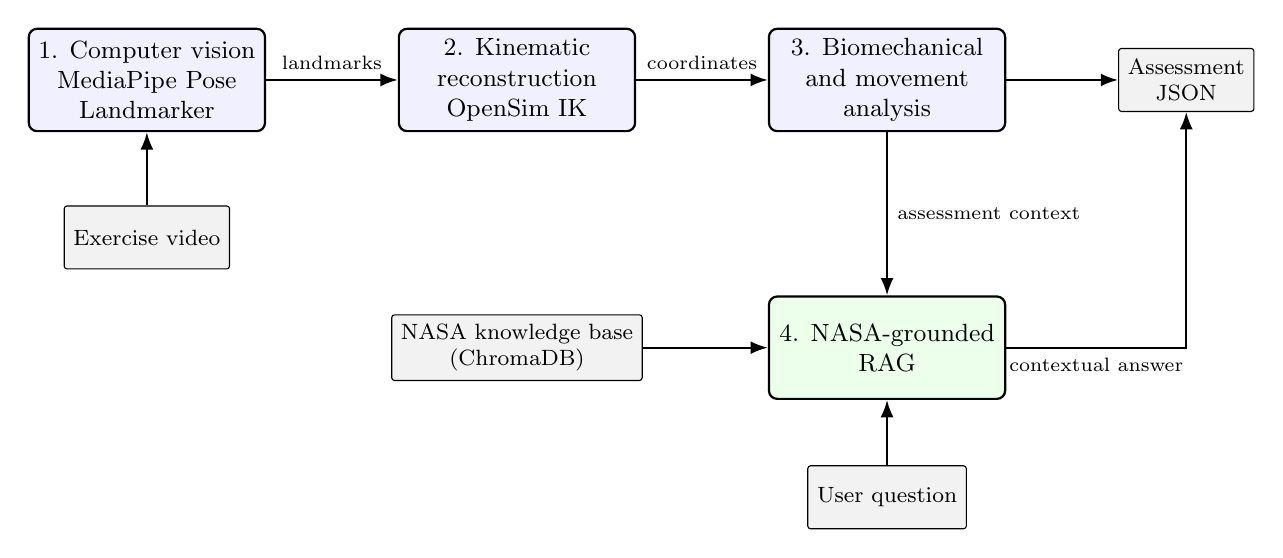
\begin{tikzpicture}
\node[stage] (cv) at (0,0) {1. Computer vision\\MediaPipe Pose\\Landmarker};
\node[stage] (ik) at (4.7,0) {2. Kinematic\\reconstruction\\OpenSim IK};
\node[stage] (bio) at (9.4,0) {3. Biomechanical\\and movement\\analysis};
\node[data] (out) at (13.2,0) {Assessment\\JSON};
\node[data] (vid) at (0,-2.0) {Exercise video};
\node[stage,fill=green!8] (rag) at (9.4,-3.4) {4. NASA-grounded\\RAG};
\node[data] (kb) at (4.7,-3.4) {NASA knowledge base\\(ChromaDB)};
\node[data] (q) at (9.4,-5.3) {User question};
\draw[arr] (vid) -- (cv);
\draw[arr] (cv) -- node[above,font=\scriptsize]{landmarks} (ik);
\draw[arr] (ik) -- node[above,font=\scriptsize]{coordinates} (bio);
\draw[arr] (bio) -- (out);
\draw[arr] (bio) -- node[right,font=\scriptsize]{assessment context} (rag);
\draw[arr] (kb) -- (rag);
\draw[arr] (q) -- (rag);
\draw[arr] (rag.east) -| node[below,font=\scriptsize,pos=0.25]{contextual answer} (out.south);
\end{tikzpicture}
\caption{\TALA\ system architecture. Stages 1--3 produce observations and model-derived estimates; Stage 4 retrieves NASA evidence and generates contextual text without modifying the numerical outputs.}
\label{fig:architecture}
\end{figure}

\begin{table}[H]
\centering
\caption{Data flow of the four \TALA\ stages.}
\label{tab:stages}
\small
\begin{tabularx}{\linewidth}{>{\raggedright\arraybackslash}p{2.6cm} >{\raggedright\arraybackslash}X >{\raggedright\arraybackslash}X >{\raggedright\arraybackslash}X}
\toprule
\textbf{Stage} & \textbf{Input} & \textbf{Processing} & \textbf{Output}\\
\midrule
Computer vision & Astronaut exercise video & \MediaPipe\ Pose Landmarker & Pose landmarks and confidence values\\
Kinematic reconstruction & Pose landmarks and selected model targets & Model scaling, target preparation, \OpenSim\ IK & Reconstructed motion, mapped coordinates, IK report\\
Biomechanical analysis & Reconstructed coordinates and scaled model & Movement analysis, COM, gravity-dependent potential energy, assessment & Movement observations, gravity report, assessment JSON\\
NASA RAG & User question and NASA knowledge base & Embedding, ChromaDB retrieval, Gemini generation & Contextual answer with source information\\
\bottomrule
\end{tabularx}
\end{table}

\subsection{Video Source and Pose Estimation}

The pilot uses publicly available astronaut exercise footage from Friends of NASA, trimmed to the squat-focused segment used in the final reconstruction. The final processed run covers 282 frames at 30 fps, corresponding to approximately 9.375 seconds of motion at a resolution of $720\times1280$ pixels. It is a single-camera source, not a calibrated motion-capture recording.

The pose-estimation stage uses the \MediaPipe\ Pose Landmarker Lite model, which returns 33 landmarks per frame; 282 frames were processed in the final workflow. A confidence threshold of 0.5 is applied to determine valid detections, and the downstream preparation logic keeps only finite, valid target samples for the IK inputs. The selected subset of landmarks (bilateral shoulders, hips, knees, ankles, heels, and foot indices) is then used to prepare the kinematic reconstruction inputs; not every \MediaPipe\ landmark is used directly by \OpenSim. Because the recording is monocular and no calibrated ground truth is available, the pose output is treated as an estimated visual observation rather than a validated anatomical reconstruction.

\subsection{OpenSim Kinematic Reconstruction}

The reconstruction proceeds as follows: (1) load the Rajagopal musculoskeletal model (\texttt{Rajagopal\allowbreak LaiUhlrich\allowbreak 2023\allowbreak.osim}); (2) scale the model according to the implemented workflow; (3) prepare pose targets from the selected video landmarks; (4) run \OpenSim\ inverse kinematics; (5) generate the reconstructed motion and coordinate outputs; and (6) produce the IK report and marker-fitting diagnostics.

The resulting three-dimensional motion is a \emph{model-constrained reconstruction}. It is not a direct three-dimensional measurement from the monocular camera: the model supplies anatomical and kinematic structure that the video alone cannot establish. In the final implementation, the pelvis translation in the camera-depth direction is held at zero (`pelvis_tx` is fixed at zero), and the unobserved right arm is neutralized with `arm_flex_r = 0`, `arm_add_r = 0`, `arm_rot_r = 0`, `elbow_flex_r = 15^\circ` (`0.2618` rad), and `pro_sup_r = 0`. No ankle coordinates are fixed at zero in the final report; the ankle coordinates are observed and fitted when the corresponding landmarks are valid. The whole body is therefore not independently reconstructed.

\subsection{Biomechanical and Movement Analysis}

\paragraph{A. Kinematic observations.} The assessment reads the mapped bilateral hip, knee, and ankle coordinates. These are model-coordinate observations, not direct measurements of muscle strength or joint loading. Coordinates in radians are converted to degrees by multiplying by $180/\pi$, and excursion is the difference between the maximum and minimum value over the analyzed samples, matching the assessment code (`coordinate_excursion_degrees = max_degrees - min_degrees`).

\paragraph{B. Center-of-mass and gravity analysis.} The scaled model provides segment masses and positions, which are used in Equation~\ref{eq:com} to estimate the whole-body center of mass. The gravity module then evaluates relative gravitational potential energy (Equation~\ref{eq:potential}) under four scenarios: microgravity ($0\,\mathrm{m/s^2}$), Moon ($1.62\,\mathrm{m/s^2}$), Mars ($3.71\,\mathrm{m/s^2}$), and Earth ($9.80665\,\mathrm{m/s^2}$). The reconstructed trajectory is held fixed across scenarios. The analysis does not calculate muscle activation, metabolic expenditure, external resistance, joint reaction forces, bone strain, or movement adaptation.

\paragraph{C. Movement assessment and daily check-in.} The movement-analysis module uses the reconstructed COM trajectory to identify repetitions and movement characteristics. The assessment module combines movement observations, IK reconstruction quality, and gravity context. It accepts optional daily check-in information and supports partial check-ins; missing values remain unavailable rather than being interpreted as normal. It checks whether a compatible personal baseline exists and produces structured JSON containing observations, context, insights, and limitations.

A personal baseline requires multiple compatible sessions from the same individual under comparable conditions. With only one compatible session, the system reports that the personal baseline is unavailable, rather than substituting a population norm or invented history.

\subsection{NASA Knowledge Base and RAG}

The knowledge base contains six NASA or NASA HRP documents \cite{nasa_std1,nasa_std2,ochmo_biomech,ochmo_exercise,hrp_fitness,hrp_sleep}, listed in Table~\ref{tab:kb}.

\begin{table}[H]
\centering
\caption{Current NASA knowledge-base and RAG configuration.}
\label{tab:kb}
\begin{tabularx}{\linewidth}{l X}
\toprule
\textbf{Item} & \textbf{Current implementation}\\
\midrule
Source documents & 6 NASA / NASA HRP documents\\
Total pages ingested & 839\\
Text chunks & 1,341\\
Embedding model & \texttt{qwen3-embedding:0.6b}\\
Embedding dimensions & 1,024\\
Vector database & ChromaDB\\
Collection & \texttt{tala\_\allowbreak nasa\_\allowbreak knowledge}\\
Similarity configuration & Cosine distance\\
Generation model & \texttt{gemini-3.5-flash-lite}\\
Retrieval output & Top 3 evidence passages (documented configuration)\\
\bottomrule
\end{tabularx}
\end{table}

The workflow (Figure~\ref{fig:rag}) is: (1) extract text from the NASA PDFs while preserving page and document metadata; (2) divide the text into overlapping chunks; (3) generate dense embeddings; (4) store embeddings and metadata in ChromaDB; (5) embed the user's question; (6) retrieve relevant chunks by cosine distance; (7) pass the retrieved passages and question to Gemini; and (8) generate a concise contextual response that retains source information. Ingestion populated the knowledge base with six documents, 839 pages, and 1,341 chunks, with no empty pages, failures, or warnings reported.

\begin{figure}[H]
\centering
\resizebox{\linewidth}{!}{%
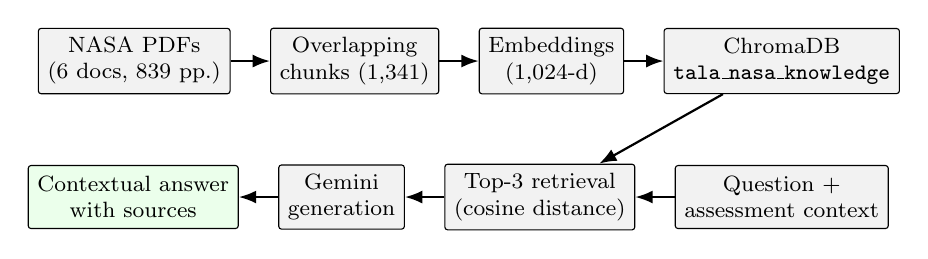
\begin{tikzpicture}[node distance=0.5cm]
\node[data] (pdf) {NASA PDFs\\(6 docs, 839 pp.)};
\node[data,right=of pdf] (chunk) {Overlapping\\chunks (1,341)};
\node[data,right=of chunk] (emb) {Embeddings\\(1,024-d)};
\node[data,right=of emb] (db) {ChromaDB\\\texttt{tala\_\allowbreak nasa\_\allowbreak knowledge}};
\node[data,below=0.9cm of db] (q) {Question +\\assessment context};
\node[data,left=of q] (ret) {Top-3 retrieval\\(cosine distance)};
\node[data,left=of ret] (gem) {Gemini\\generation};
\node[data,left=of gem,fill=green!8] (ans) {Contextual answer\\with sources};
\draw[arr] (pdf)--(chunk); \draw[arr] (chunk)--(emb); \draw[arr] (emb)--(db);
\draw[arr] (q)--(ret); \draw[arr] (db)--(ret); \draw[arr] (ret)--(gem); \draw[arr] (gem)--(ans);
\end{tikzpicture}}
\caption{NASA knowledge-base ingestion (top) and retrieval-augmented generation (bottom).}
\label{fig:rag}
\end{figure}

The role of this component is bounded:
\begin{quote}
The RAG component provides literature-based context for interpreting assessment outputs. It does not calculate biomechanical quantities, change assessment flags, establish clinical thresholds, or diagnose a medical condition.
\end{quote}
No retrieval-accuracy or hallucination rate is measured in this paper, because no formally labeled evaluation benchmark exists yet.

\subsection{Software Implementation and Testing}

The backend is implemented in Python with configuration-driven processing. The unified pipeline is executed through \texttt{scripts/\allowbreak run\_\allowbreak tala.py}, and the knowledge base is built with \texttt{scripts/\allowbreak build\_\allowbreak knowledge\_\allowbreak base.py}. The structured assessment is written to \texttt{results/\allowbreak tala\_\allowbreak output.json}, alongside the reconstruction, gravity, and movement artifacts. The current repository checkout is on the `main` branch at commit `300edea630e8e935b87f78e075f7d989a11bd95f` with no formal release tag in the working tree; the local environment is Python 3.11.9 on Windows 10 (Intel64), with NumPy 2.3.5, pandas 2.3.3, and pytest 8.4.2 installed.

\section{Experimental Results}

This section reports only the results currently available from the implementation. It does not include human-subject validation, motion-capture comparison, force-plate testing, clinical assessment, or a formal RAG benchmark.

\subsection{Computer-Vision Pose-Estimation Results}

\begin{table}[H]
\centering
\caption{Pose-estimation output for the exercise recording.}
\label{tab:pose}
\begin{tabular}{lr}
\toprule
\textbf{Metric} & \textbf{Result}\\
\midrule
Video duration & Approximately 9.375 s\\
Resolution & $720\times1280$\\
Frame-rate metadata & 30 fps\\
Processed frames & 282\\
Successful pose detections & 282 / 282\\
Landmarks per frame & 33\\
Total landmark records & 9,306\\
Frames with all selected landmarks valid & 282\\
Confidence threshold & 0.5\\
\bottomrule
\end{tabular}
\end{table}

All 282 frames received a pose detection, and the final selected target set remained valid for all processed frames in the current reconstruction. A successful detection rate should therefore not be equated with complete landmark quality: the detector can return a pose in which some landmarks needed downstream are below the confidence threshold or occluded, and the final IK mapping intentionally omits unobserved limbs rather than fabricating movement. Figure~\ref{fig:cvos}(a) shows the detected landmarks overlaid on a source frame.

\subsection{OpenSim Kinematic Reconstruction Results}

Table~\ref{tab:coords} summarizes the bilateral joint-coordinate ranges from the final reconstruction run, and Figure~\ref{fig:sequence} shows reconstructed model poses across the movement. The final reconstruction used 282 samples (9.375 s at the recorded sampling rate), the marker-fitting report indicates a mean error of about 0.0265 m, an RMS error of about 0.0306 m, and a maximum error of about 0.1377 m, and each frame had 12 valid IK markers in the final target set.

\begin{table}[H]
\centering
\caption{Selected bilateral model-coordinate ranges from the final reconstruction (\texttt{ik\_\allowbreak report.json}). These are model coordinates, not clinical range-of-motion measurements.}
\label{tab:coords}
\begin{tabular}{lrrl}
\toprule
\textbf{Coordinate} & \textbf{Minimum} & \textbf{Maximum} & \textbf{Units}\\
\midrule
Right hip & 0.0991 & 2.0903 & rad\\
Left hip & 0.3620 & 1.9484 & rad\\
Right knee & 0.0028 & 2.4425 & rad\\
Left knee & 0.1323 & 2.4377 & rad\\
Right ankle & -0.8458 & -0.0517 & rad\\
Left ankle & -0.8148 & -0.0971 & rad\\
\bottomrule
\end{tabular}
\end{table}

The ankle coordinates are not fixed at zero in the final reconstruction; they are fitted from the valid ankle landmarks and should be interpreted as model-based coordinate estimates, not as independent anatomical measurements.

\subsection{Visual Comparison: MediaPipe Versus OpenSim}

Figure~\ref{fig:cvos} shows the central transformation in the pipeline: a visual observation from computer vision and the corresponding model-based reconstruction at the same movement frame.

\begin{figure}[H]
\centering
\begin{subfigure}[b]{0.48\linewidth}\centering
\figorbox[\linewidth]{fig2a_mediapipe_frame.png}{Original frame with MediaPipe landmarks and skeleton}
\caption{Computer vision: visual observation}
\end{subfigure}\hfill
\begin{subfigure}[b]{0.48\linewidth}\centering
\figorbox[\linewidth]{fig2b_opensim_frame.png}{OpenSim reconstructed pose, same timestamp}
\caption{OpenSim: model-based reconstruction}
\end{subfigure}
\caption{Computer-vision pose estimation versus OpenSim kinematic reconstruction at the same movement frame. The right panel is generated through musculoskeletal-model constraints and is not a direct camera measurement of three-dimensional anatomy.}
\label{fig:cvos}
\end{figure}

\begin{figure}[H]
\centering
\figorbox{fig3_reconstructed_squat_sequence.png}{Four reconstructed model poses: upright, descent, deepest position, ascent}
\caption{Reconstructed squat sequence showing four model poses (upright, descent, deepest position, ascent). These are reconstructed model poses, not camera measurements.}
\label{fig:sequence}
\end{figure}

\subsection{Movement-Analysis Results}

\begin{table}[H]
\centering
\caption{Movement-analysis results from the latest unified assessment.}
\label{tab:movement}
\begin{tabular}{lr}
\toprule
\textbf{Metric} & \textbf{Latest reported result}\\
\midrule
Exercise & Squat\\
Samples & 282\\
Detected repetitions & 2\\
Movement completeness & Incomplete\\
COM vertical range & Approximately 0.8917--1.5671 m\\
Right hip excursion & $114.09^\circ$\\
Left hip excursion & $90.89^\circ$\\
Compatible personal baseline & Unavailable\\
\bottomrule
\end{tabular}
\end{table}

The analysis detected two repetitions, and movement completeness was reported as incomplete. The recording therefore should not be interpreted as a complete exercise session or workout. Figure~\ref{fig:com} shows the vertical COM trajectory with the detected upper and lower positions that define the two repetitions. The reported hip excursions are derived from model coordinates, as described in the methodology, and are not clinical range-of-motion measurements.

\begin{figure}[H]
\centering
\figorbox{fig4_com_trajectory.png}{Vertical COM position (m) vs time (s), annotated with detected upper/lower positions}
\caption{Vertical center-of-mass trajectory over time, annotated with the upper and lower movement positions identified by the movement-analysis module.}
\label{fig:com}
\end{figure}

\subsection{Gravity-Dependent Potential-Energy Results}

\begin{table}[H]
\centering
\caption{Gravity conditions and relative gravitational potential-energy results for the same reconstructed trajectory. Values must be taken from the final \texttt{gravity\_\allowbreak analysis.json}.}
\label{tab:gravity}
\small
\begin{tabular}{lrrrr}
\toprule
\textbf{Output} & \textbf{Microgravity} & \textbf{Moon} & \textbf{Mars} & \textbf{Earth}\\
\midrule
Gravity (m/s$^2$) & 0 & 1.62 & 3.71 & 9.80665\\
Minimum relative PE (J) & 0.00 & -23.12 & -52.95 & -139.97\\
Maximum relative PE (J) & 0.00 & 59.23 & 135.65 & 358.57\\
PE range (J) & 0.00 & 82.36 & 188.60 & 498.54\\
\bottomrule
\end{tabular}
\end{table}

The final gravity analysis used a total modeled body mass of $74.3044\,\mathrm{kg}$ and a COM height excursion of $0.6842\,\mathrm{m}$ over the analyzed trajectory; these values are taken directly from the final `gravity_analysis.json` report.

Because the trajectory and modeled mass are held fixed, the potential-energy results scale with gravity (Figure~\ref{fig:pe}). They should not be interpreted as measured muscular effort or energy expenditure.

\begin{figure}[H]
\centering
\figorbox{fig5_gravity_pe.png}{Relative PE (J) vs time (s) for microgravity, Moon, Mars, Earth}
\caption{Relative gravitational potential energy versus time for microgravity, Moon, Mars, and Earth. The same reconstructed trajectory is used for every gravity scenario.}
\label{fig:pe}
\end{figure}

\subsection{Assessment and RAG Results}

The unified runner generated a structured assessment. The latest run identified the exercise as a squat, detected two repetitions, and reported movement completeness as incomplete. The personal baseline was unavailable because only one compatible session existed. The NASA knowledge base contained six documents, 839 pages, and 1,341 chunks, and the integrated RAG generation stage was available in the latest unified run.

Any screenshot of the assessment JSON or frontend display should be labeled as either (i) a live backend result generated by the unified runner or (ii) a prepared example response used in the frontend demonstration. Prepared responses are demonstration examples and are not live RAG queries.

\subsection{Software Test Results}

\begin{table}[H]
\centering
\caption{Automated software test result.}
\label{tab:tests}
\begin{tabular}{lr}
\toprule
\textbf{Test result} & \textbf{Value}\\
\midrule
Automated tests passed & 8\\
Execution time & 20.76 s\\
\bottomrule
\end{tabular}
\end{table}

These tests support software-level verification, not scientific or clinical validity.

\begin{table}[H]
\centering
\caption{Implementation status of the major \TALA\ components.}
\label{tab:status}
\begin{tabularx}{\linewidth}{l l X}
\toprule
\textbf{Component} & \textbf{Status} & \textbf{Evidence / qualification}\\
\midrule
Video pose extraction & Implemented & 282 frames processed; 33 landmarks per frame\\
OpenSim kinematic reconstruction & Implemented & Model-constrained reconstruction and IK report\\
Movement and COM analysis & Implemented & Squat, 2 repetitions detected, incomplete\\
Gravity potential-energy analysis & Implemented & Fixed-trajectory comparison\\
NASA-document RAG & Implemented & 6 documents, 1,341 chunks; no formal benchmark\\
Longitudinal personal baseline & Unavailable & Only one compatible session\\
Clinical or astronaut validation & Not performed & Requires independent reference data and approval\\
\bottomrule
\end{tabularx}
\end{table}

\section{Discussion}

\subsection{Feasibility of Video-Based Movement Observation}

All processed frames received a pose detection in the current run, yet the selected target set is still limited by monocular depth ambiguity and partial limb visibility. This shows that monocular video provides useful movement observations but that detection success is not a measure of anatomical quality or complete kinematic observability. Monocular video cannot independently establish accurate three-dimensional anatomical motion.

\subsection{Model-Constrained Kinematic Reconstruction}

\OpenSim\ provides a structured musculoskeletal representation for interpreting the visual observations. Reconstruction quality depends on the selected landmarks, model scaling, coordinate mapping, and the available observations, and the reconstructed motion should be read as informed by the video rather than measured from it.

\subsection{Biomechanical Interpretation Under Different Gravity Conditions}

Comparing potential-energy changes under different gravity magnitudes illustrates how a gravity-dependent quantity scales with $g$ for a given COM trajectory. This is a fixed-trajectory computational comparison, not a prediction of how an astronaut would exercise in another gravitational environment.

\subsection{NASA Literature Contextualization}

RAG makes relevant NASA documents accessible alongside the assessment. It provides contextual information, but the quality of an answer depends on retrieval relevance and on the support available in the retrieved passages.

Overall, the contribution of this work is the integration of these stages into one reproducible workflow, not the discovery of a new clinical measurement or a validated astronaut-health predictor. Video-derived observations, model-based kinematic outputs, gravity context, and literature remain distinguishable by provenance, and a single session is not presented as a personal trend.

\section{Limitations and Threats to Validity}

Several limitations constrain the conclusions of this study.

\begin{enumerate}[label=\arabic*.]
  \item \textbf{Monocular camera.} A single camera introduces perspective and depth ambiguity.
  \item \textbf{No motion-capture ground truth.} There is no calibrated reference dataset to quantify reconstruction accuracy.
  \item \textbf{Pose-estimation uncertainty.} Landmark confidence and visibility do not guarantee anatomical correctness.
  \item \textbf{Model dependence.} \OpenSim\ outputs depend on the selected model, scaling, coordinate mapping, and assumptions.
  \item \textbf{Incomplete coordinate observation.} Not all body degrees of freedom are independently observed or reconstructed.
  \item \textbf{Incomplete recording.} The current squat segment is not a complete exercise session.
  \item \textbf{Fixed-trajectory gravity comparison.} The gravity scenarios do not model behavioral or physiological adaptation.
  \item \textbf{Limited longitudinal data.} One compatible session is insufficient to establish a personal baseline or trend.
  \item \textbf{No clinical validation.} The outputs do not diagnose, predict injury, establish medical readiness, or provide treatment recommendations. The system does not perform inverse dynamics and does not estimate joint moments or muscle activation.
  \item \textbf{RAG evaluation.} There is no manually labeled retrieval-quality benchmark yet.
  \item \textbf{Frontend demonstration.} Prepared interface examples must not be represented as live backend measurements or live RAG responses.
\end{enumerate}

\begin{quote}
The three-dimensional kinematic output should be interpreted as a model-constrained reconstruction informed by monocular visual observations, rather than as an independently measured representation of the subject's anatomical motion. Consequently, downstream biomechanical quantities inherit uncertainty from both the visual input and the musculoskeletal model assumptions.
\end{quote}

\section{Conclusion and Future Work}

This paper presented \TALA, an exploratory framework that connects video-based pose extraction, \OpenSim\ kinematic reconstruction, biomechanical and movement analysis, and NASA-literature-grounded RAG, integrated into a structured assessment. The current backend processed 282 frames of a squat recording, reconstructed model-constrained kinematics, analyzed center-of-mass behavior and gravity-dependent potential energy, identified two repetitions, and provided a knowledge base of six NASA documents (1,341 chunks) for contextual retrieval.

The results are preliminary. The pose experiment uses a single monocular recording without independent ground truth, the recording is incomplete, gravity-dependent energy values are computational comparisons of a fixed trajectory, and the RAG component has not undergone a formal benchmark. \TALA\ should therefore be regarded as a research and demonstration prototype rather than a validated astronaut-health monitoring system.

Future work should (i) validate the kinematic reconstruction against calibrated motion-capture data; (ii) improve camera calibration and pursue multi-view reconstruction; (iii) evaluate coordinate mapping and reconstruction errors; (iv) expand compatible exercise sessions for longitudinal comparison; (v) establish a manually verified RAG evaluation dataset; and (vi) evaluate the system with more representative astronaut exercise recordings.

\section*{Acknowledgments}
This project was developed as a repository-based research prototype using the current TALA codebase, generated result files, and NASA literature sources included in the project. The author acknowledges the Friends of NASA source video and the project contributors reflected in the repository history and generated artifacts, without claiming a formal institutional sponsor or external advisory body beyond the current repository state.

\section*{Data and Code Availability}
The implementation and generated artifacts are maintained in the TALA project repository at \url{https://github.com/Arxivory/tala}. The current working-tree checkout is on the `main` branch at commit `300edea630e8e935b87f78e075f7d989a11bd95f`; no formal release tag is present in this local checkout. The source video is publicly available from Friends of NASA; the repository does not redistribute the raw video, so the original source page and access date should be recorded with the final dataset citation. Model files and NASA documents should be referenced by their official source locations and versions.

\begin{thebibliography}{99}

\bibitem{delp2007}
S. L. Delp et al.,
``OpenSim: Open-source software to create and analyze dynamic simulations of movement,''
\emph{IEEE Transactions on Biomedical Engineering}, vol. 54, no. 11, pp. 1940--1950, 2007.

\bibitem{seth2018}
A. Seth et al.,
``OpenSim: Simulating musculoskeletal dynamics and neuromuscular control to study human and animal movement,''
\emph{PLOS Computational Biology}, vol. 14, no. 7, e1006223, 2018.

\bibitem{bazarevsky2020}
V. Bazarevsky et al.,
``BlazePose: On-device real-time body pose tracking,''
arXiv:2006.10204, 2020.

\bibitem{mediapipe}
Google,
``MediaPipe Pose Landmarker,''
\url{https://ai.google.dev/edge/mediapipe/solutions/vision/pose_landmarker}.
\placeholder{Verify documentation version and access date.}

\bibitem{lewis2020rag}
P. Lewis et al.,
``Retrieval-augmented generation for knowledge-intensive NLP tasks,''
in \emph{Advances in Neural Information Processing Systems}, vol. 33, 2020.

\bibitem{nasa_std1}
National Aeronautics and Space Administration,
\emph{NASA-STD-3001, Volume 1: Crew Health}, Revision C.
\placeholder{Verify official publication date, full title, and URL from the PDF.}

\bibitem{nasa_std2}
National Aeronautics and Space Administration,
\emph{NASA-STD-3001, Volume 2: Human Factors, Habitability, and Environmental Health}, Revision F.
\placeholder{Verify formal title, publication date, and URL from the PDF.}

\bibitem{ochmo_biomech}
NASA Office of the Chief Health and Medical Officer,
\emph{OCHMO-HB-004: Anthropometry, Biomechanics, and Strength}.
\placeholder{Verify revision/date and official URL.}

\bibitem{ochmo_exercise}
NASA Office of the Chief Health and Medical Officer,
\emph{OCHMO-TB-031: Exercise Overview: Astronaut Physiological Deconditioning and Exercise Prescription Countermeasures in Spaceflight}.
\placeholder{Verify publication date and official URL.}

\bibitem{hrp_fitness}
NASA Human Research Program,
\emph{Evidence Report: Reduced Cardiorespiratory and Musculoskeletal Fitness}.
\placeholder{Verify report identifier, revision, and URL.}

\bibitem{hrp_sleep}
NASA Human Research Program,
\emph{Evidence Report: Sleep Loss, Circadian Desynchronization, and Work Overload}.
\placeholder{Verify report identifier, revision, and URL.}

\bibitem{featherstone2008}
R. Featherstone,
\emph{Rigid Body Dynamics Algorithms}.
Springer, 2008.

\end{thebibliography}

\end{document}